\documentclass{beamer}
\usepackage[]{multirow}
\usepackage[]{array}
\usepackage[]{graphicx}
\usepackage[T1]{fontenc}
\usepackage[]{url}

\usetheme{default}
\setbeamertemplate{navigation symbols}{}

\title{Building a Raspberry Pi-Based\\Guitar Environmental Monitor}
\author{Grant Alphenaar}
\institute{CIS 641 -- GVSU}
\date{\today}

\begin{document}

  \newcommand{\sectitle}{}

  \begin{frame}
      \titlepage
  \end{frame}

  % Introduction slide
  \renewcommand{\sectitle}{Introduction \& Overview}
  \section{\sectitle}

    \begin{frame}{Roadmap}
      \tableofcontents
    \end{frame}

    \begin{frame}{\sectitle}{Project Overview}
      \begin{columns}
        \begin{column}{.5\textwidth}
          Goal: build a system that can\dots
          \begin{itemize}
            \item \dots be run off a Raspberry Pi.
            \item \dots monitor temp and humidity for guitars.
            \item \dots allow user monitoring and (some) control.
          \end{itemize}
        \end{column}
        \begin{column}{.5\textwidth}
          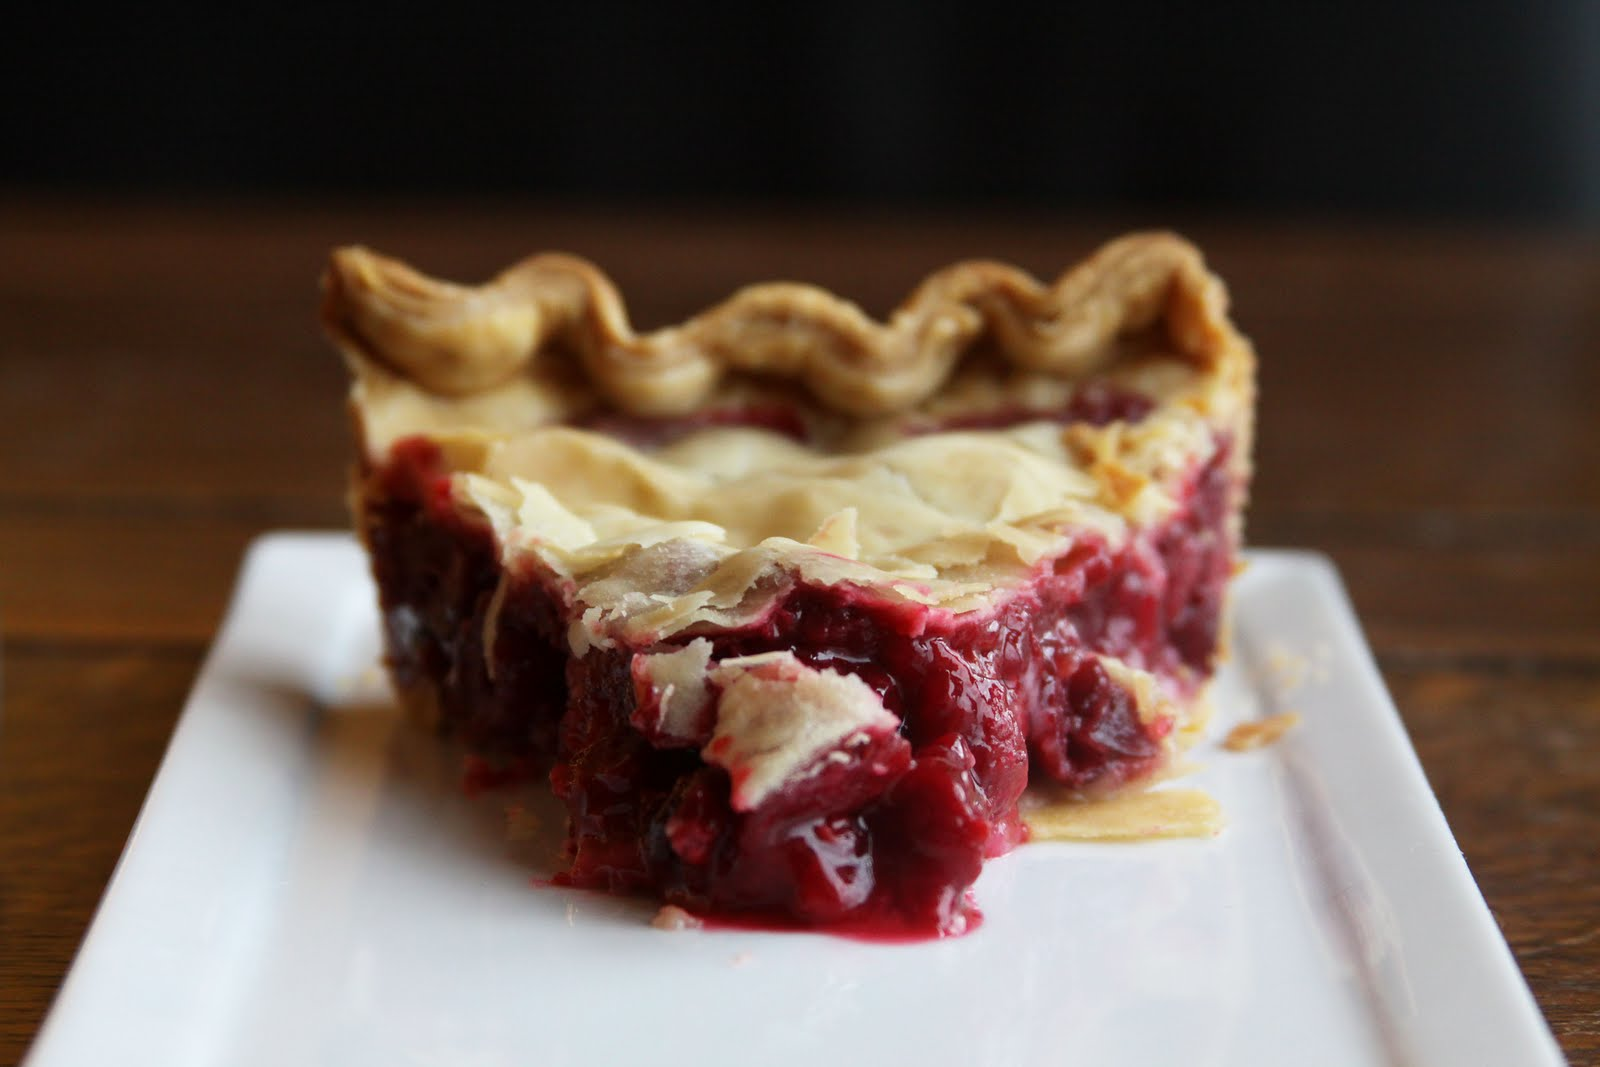
\includegraphics[scale=.09]{images/raspberry-pie.jpg}
        \end{column}
      \end{columns}
      \vspace*{\fill}
      {\tiny{source: \url{https://www.espressoandcream.com/2011/07/wedding-pie-1-cran-raspberry-pie.html} -- bonus: this website also appears to have a pretty good recipe for \textit{actual} raspberry pie}}
    \end{frame}

    \begin{frame}{\sectitle}{What?}
      \begin{center}
        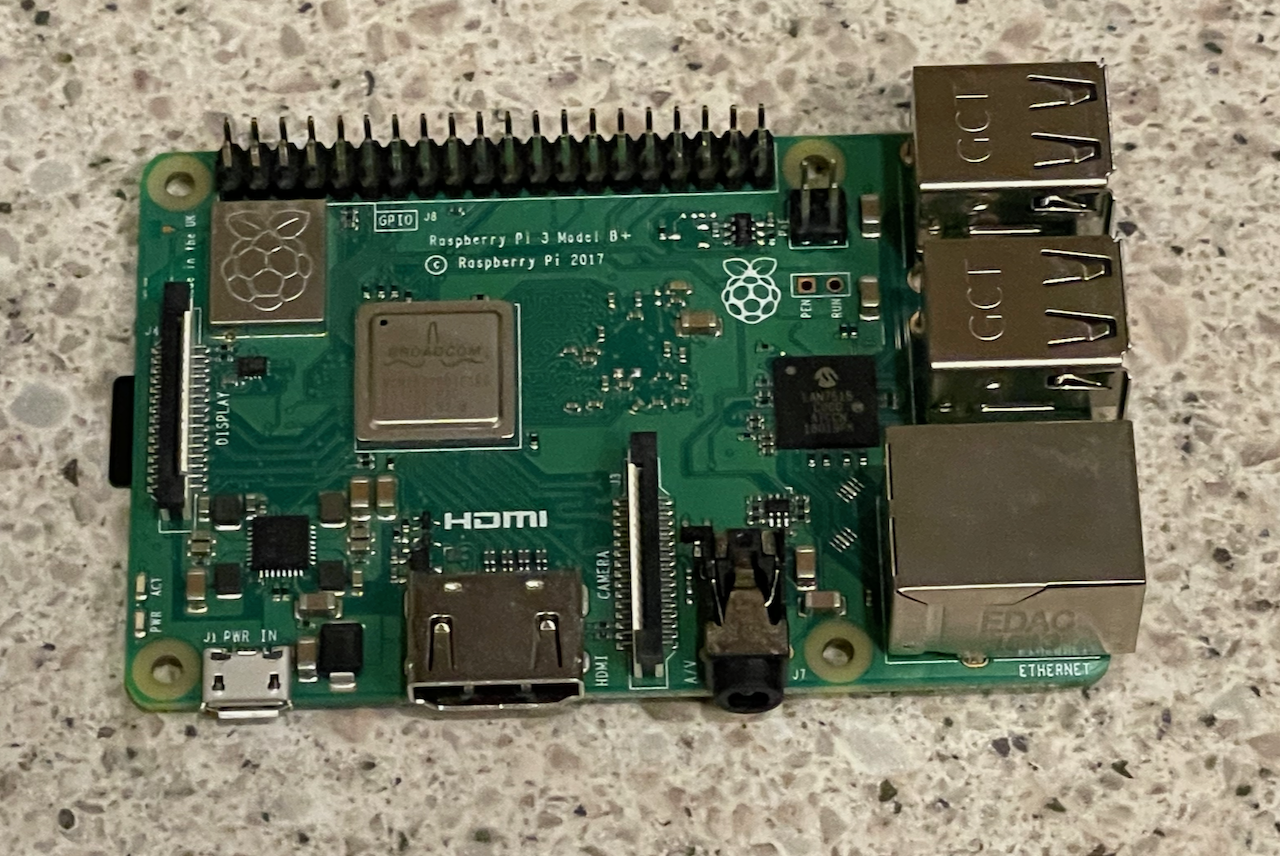
\includegraphics[scale=.20]{images/rpi.png}
      \end{center}
    \end{frame}


  \renewcommand{\sectitle}{A Bit More Detail\dots}
  \section{\sectitle}
  \begin{frame}{Roadmap}
      \tableofcontents[currentsection]
  \end{frame}

  \begin{frame}{\sectitle}{Why?}
    \begin{itemize}\LARGE
      \item Guitars are (mostly) made out of wood, and\dots
      \item \dots wood is sensitive to temperature and humidity\dots
      \item \dots especially swings to either extreme\dots
      \item \dots which Michigan has a lot of.
    \end{itemize}
  \end{frame}

  \begin{frame}{\sectitle}{Components}
    \begin{columns}
      \begin{column}{.5\textwidth}
        \centering Sensor Unit:
        \vspace*{1em}
        \begin{center}
          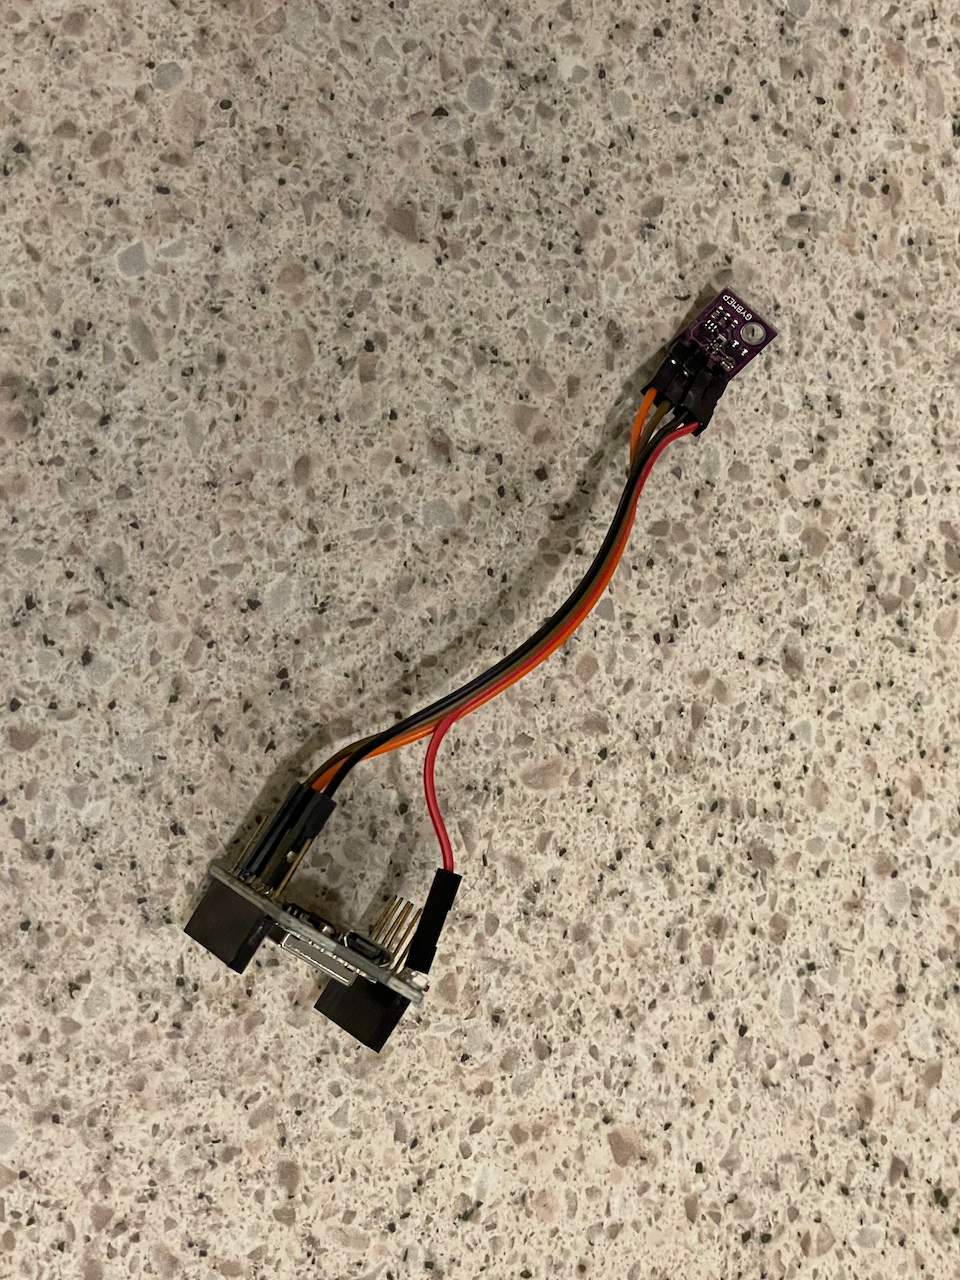
\includegraphics[scale=.1]{images/bme.png}
        \end{center}
      \end{column}
      \begin{column}{.5\textwidth}
        \centering Battery Board:
        \vspace*{1em}
        \begin{center}
          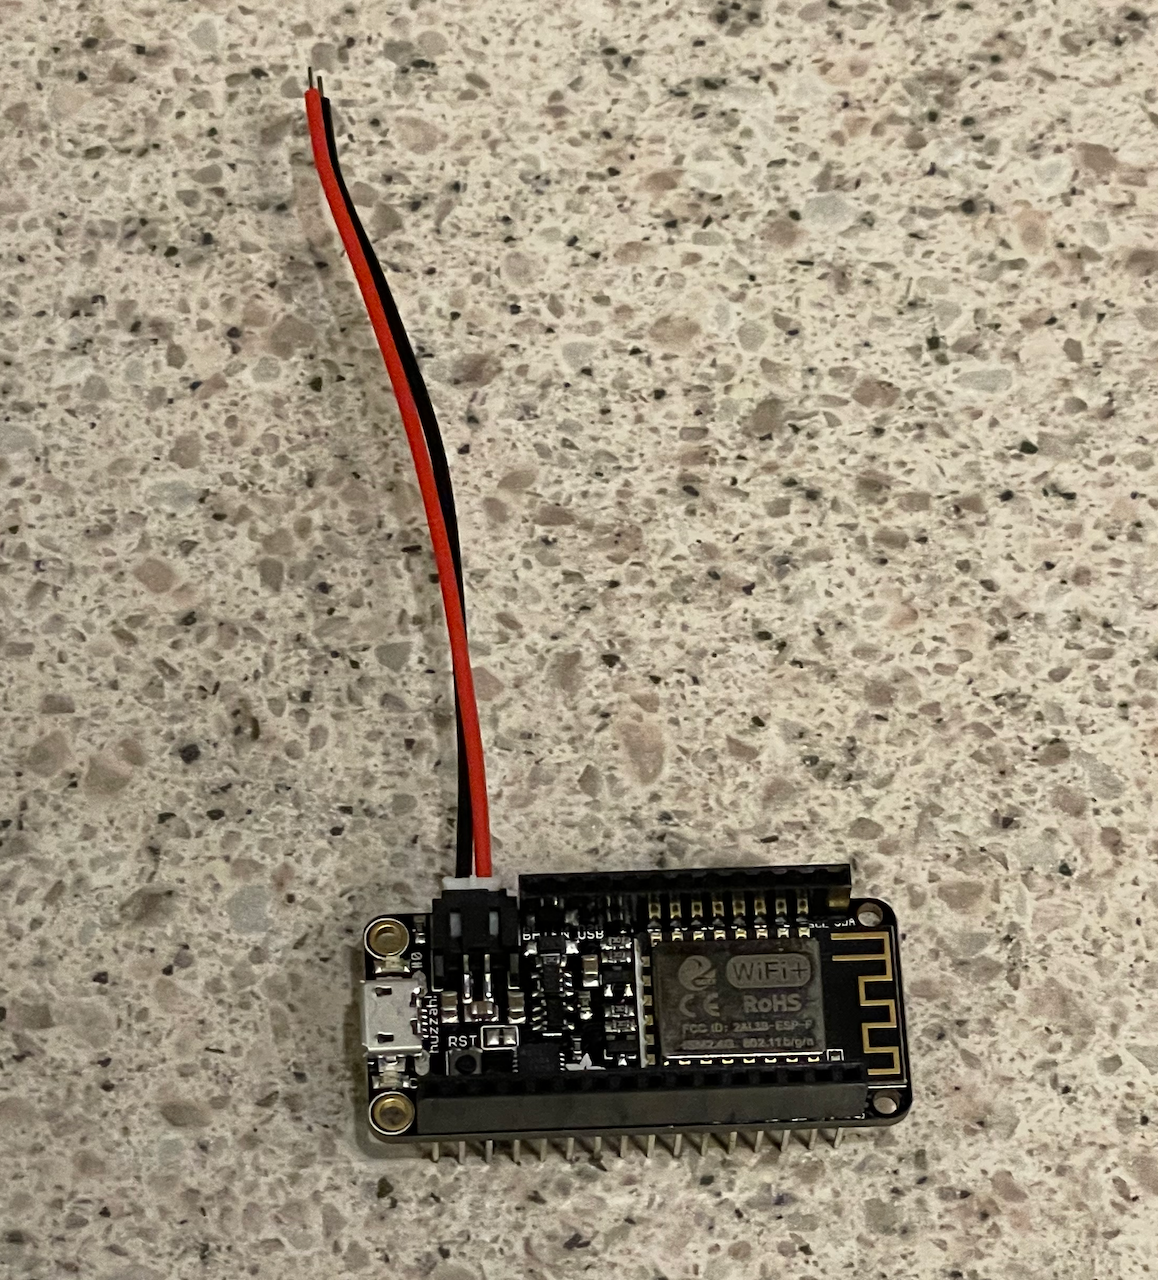
\includegraphics[scale=.1]{images/battery.png}
        \end{center}
      \end{column}
    \end{columns}
  \end{frame}


  \renewcommand{\sectitle}{Timeline}
  \section{\sectitle}
  \begin{frame}{Roadmap}
      \tableofcontents[currentsection]
  \end{frame}

  \begin{frame}{\sectitle}{}
    \begin{center}
      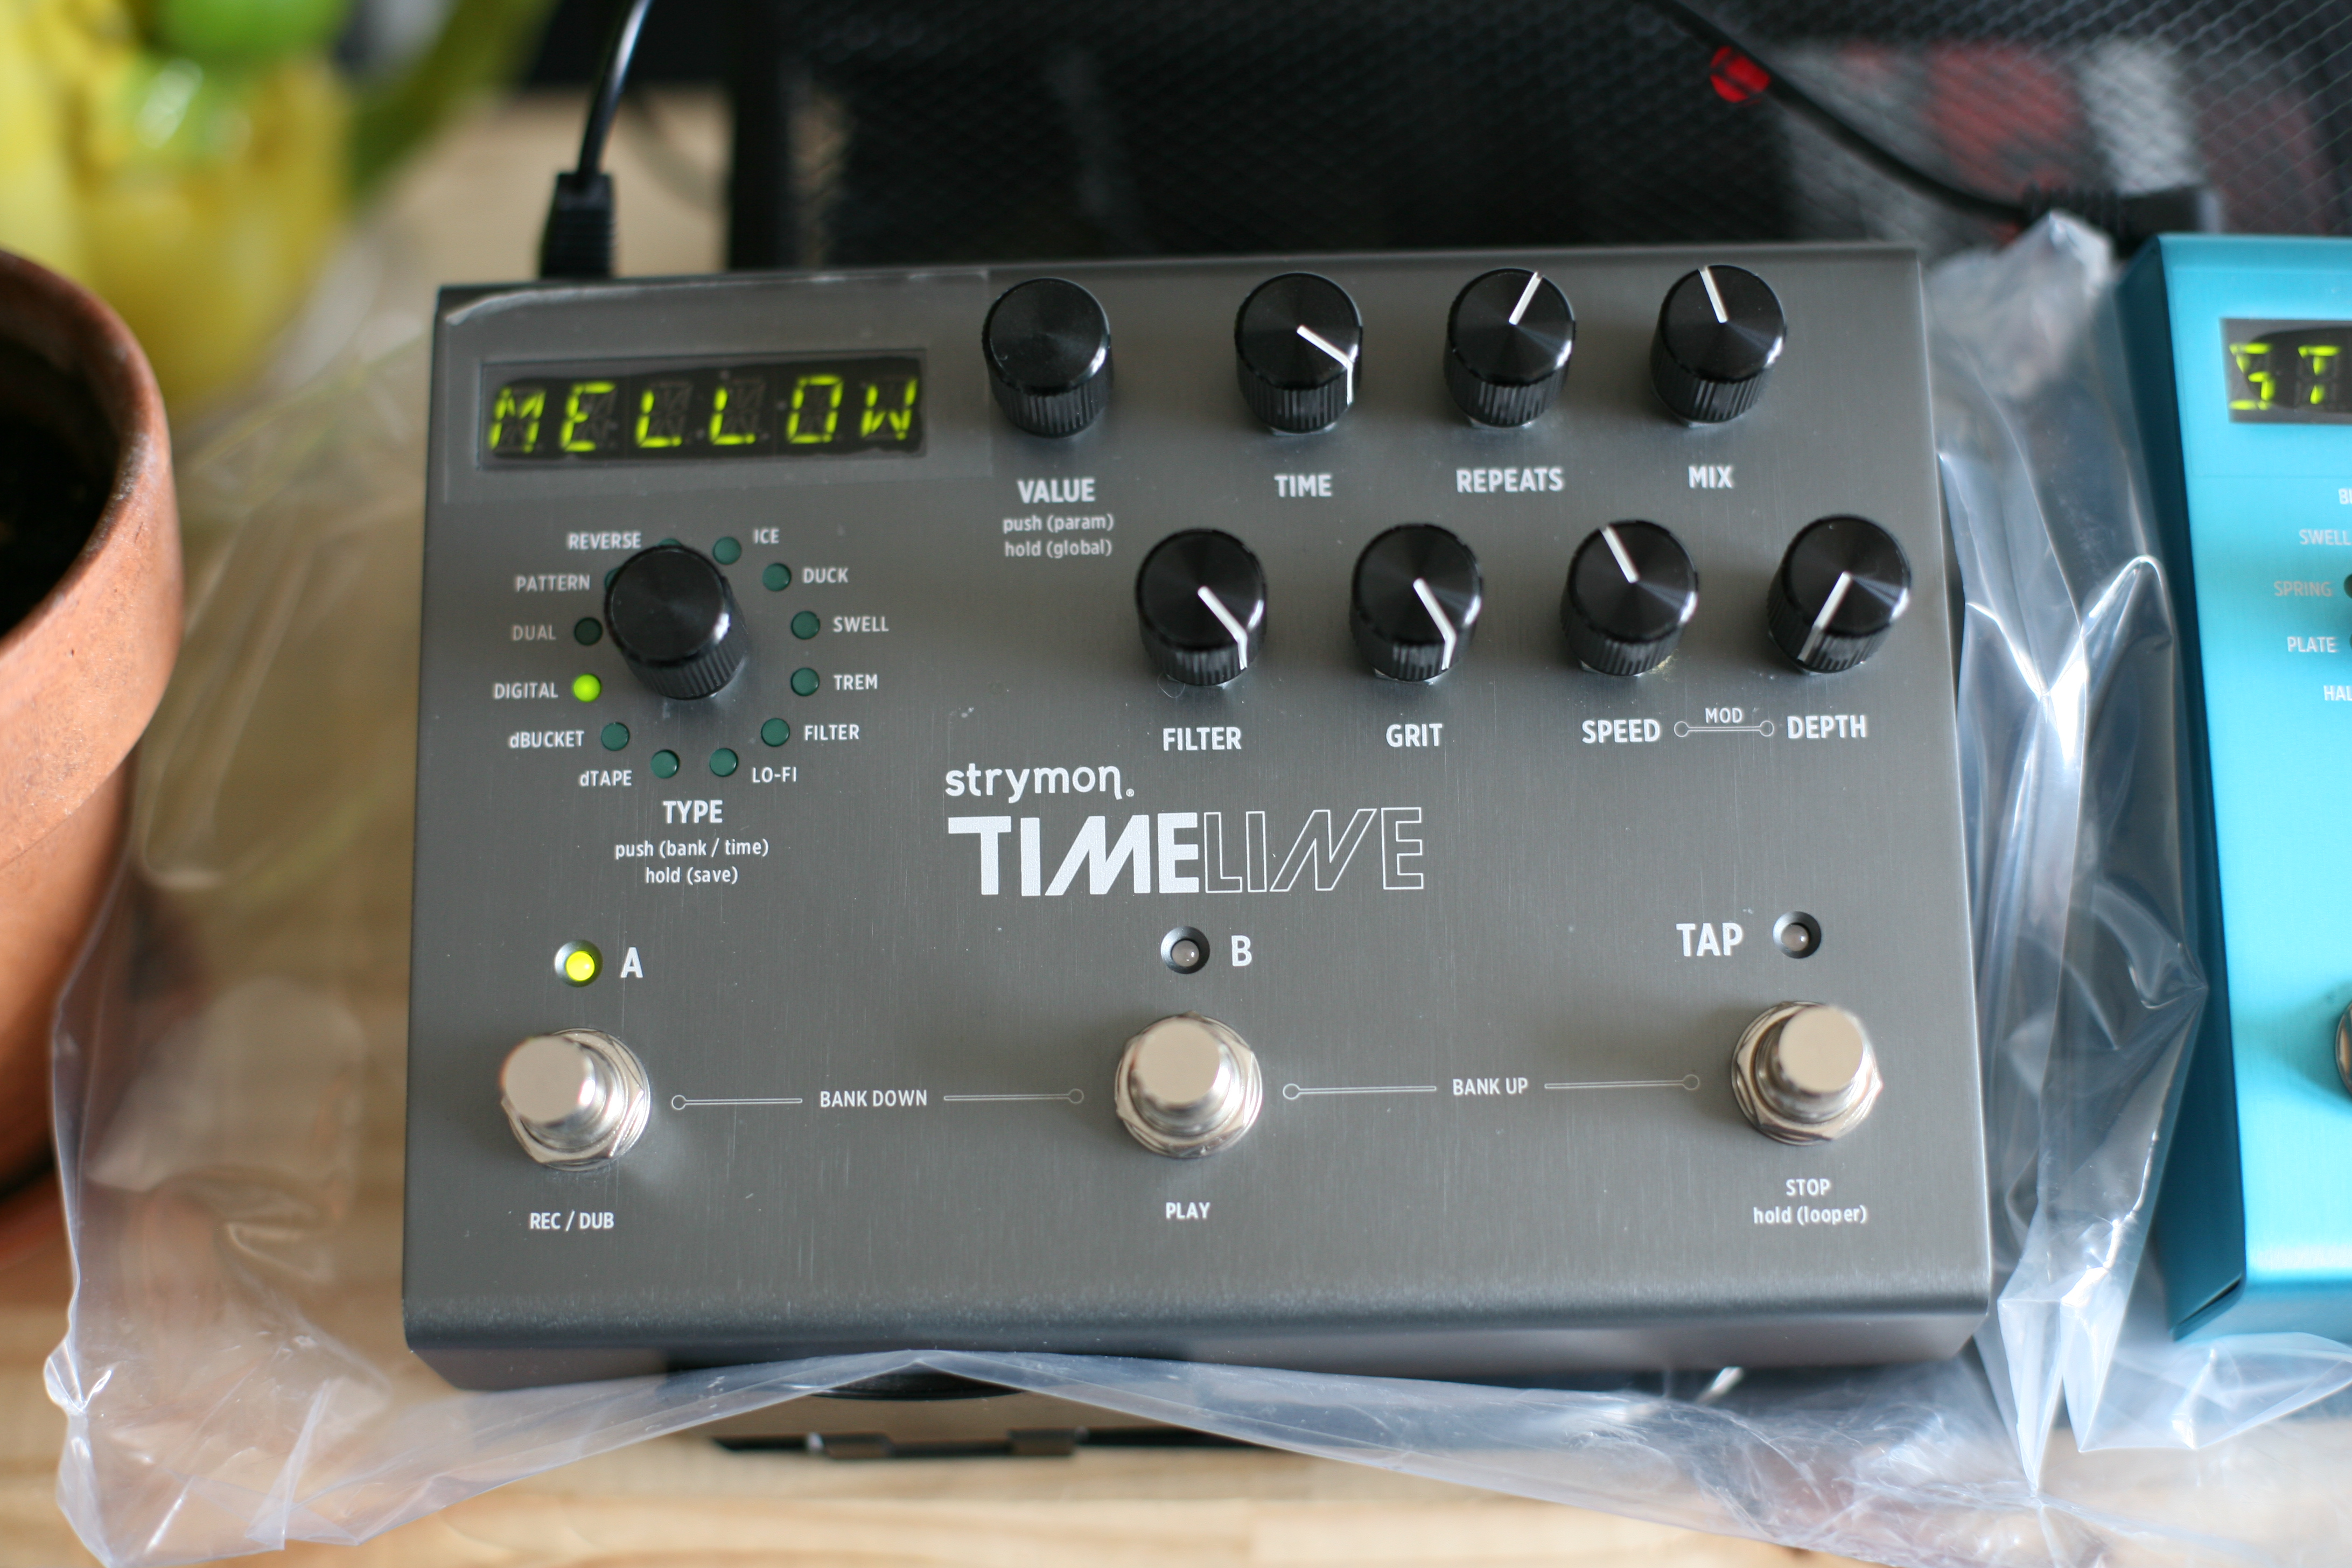
\includegraphics[scale=.07]{images/timeline.jpg}
      \tiny source: \url{https://fr.audiofanzine.com/delay-guitare/strymon/timeline/}
    \end{center}
  \end{frame}

  \begin{frame}{\sectitle}{Burn-Up}
    \begin{center}
      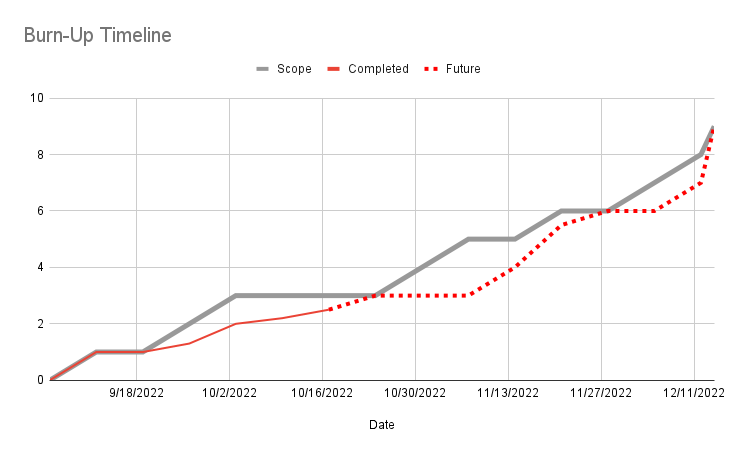
\includegraphics[scale=.4]{images/burn-up.png}
    \end{center}
  \end{frame}

  \begin{frame}{\sectitle}{Key Points}
    \begin{itemize}
      \item Early October -- End of October: sensor prototyping and finalize code for sensor ($\approx 1-2$ more weeks)
      \item Early November: Build backend and analysis capabilities ($\approx 1-2$ weeks)
      \item Late November: Build frontend -- user interface ($\approx 2-3$ weeks)
      \item Early December: Bring everything together + final touches ($\approx 1$ week)
    \end{itemize}
  \end{frame}


  \renewcommand{\sectitle}{Use Case Description, Activity Diagram, and Requirements}
  \section{\sectitle}
  \begin{frame}{Roadmap}
    \tableofcontents[currentsection]
  \end{frame}

  \begin{frame}{\sectitle}{Use Case Description}
    Use Case Name: Monitor Environment\\
    Importance Level: Critical\\
    Primary Actor: Sensor\\
    Use Case Type: Essential Overview\\
    \vspace*{1em}
    Brief Description: This use case describes the process of a Sensor taking environmental readings, logging them, and sending them to the Base Unit to be included in the web dashboard.
  \end{frame}

  \begin{frame}{\sectitle}{Use Case Description}
    Trigger:
    \begin{itemize}
      \item Event: Base Unit triggers Sensor
      \item Type: Internal
    \end{itemize}
    \vspace*{1em}
    Relationships:
    \begin{itemize}
      \item Actors:
      \begin{itemize}
        \item Base Unit
        \item Sensor
      \end{itemize}
      \item Include:
      \begin{itemize}
        \item \textit{Monitor Environment} includes \textit{Monitor Temperature} and \textit{Monitor Humidity}
      \end{itemize}
    \end{itemize}
  \end{frame}

  \begin{frame}{\sectitle}{Use Case Description}
    {\centering{Normal Flow of Events}\par}
    \begin{enumerate}
      \item Sensor is triggered
      \item Sensor takes environmental reading
      \item Sensor sends data to Base Station
      \item Base Station analyzes data and adds to database
      \item Web server reads from database and updates dashboard
      \item If\dots
      \begin{itemize}
        \item \dots reading is above safe range: alert user
        \item \dots reading is below safe range: alert user
        \item \dots continue on
      \end{itemize}
      \item (Loop begins again)
    \end{enumerate}
  \end{frame}

  \begin{frame}{\sectitle}{Use Case Description}
    {\centering{Alternate and/or Exceptional Flows}\par}
    \begin{enumerate}
      \item Server crashes: user gets default browser error message
      \item Other server faults: user gets message with resolution suggestions
      \item Sensor is offline: user gets alert if sensor cannot be triggered three times in a row
    \end{enumerate}
  \end{frame}

  % \begin{frame}{\sectitle}{Use Case Diagram}
  %   \begin{center}
  %     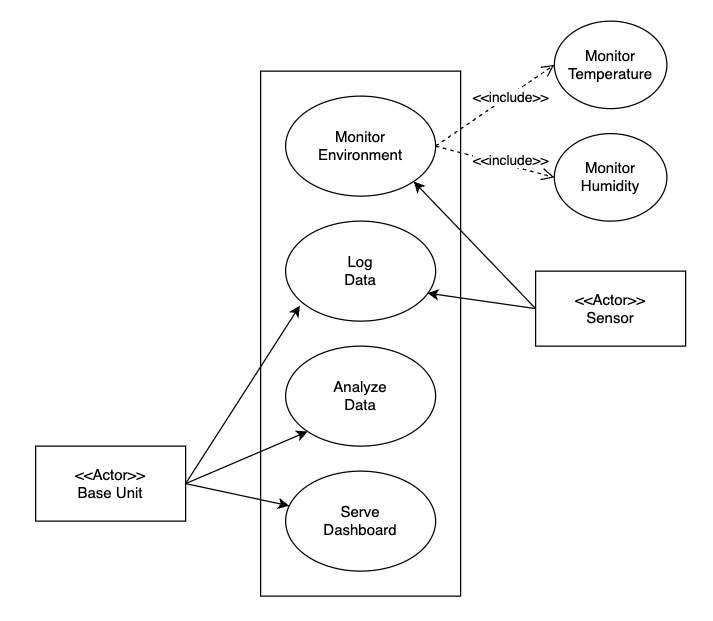
\includegraphics[scale=.35]{images/UCD.png}
  %   \end{center}
  % \end{frame}

  \begin{frame}{\sectitle}{Activity Diagram}
    \begin{center}
      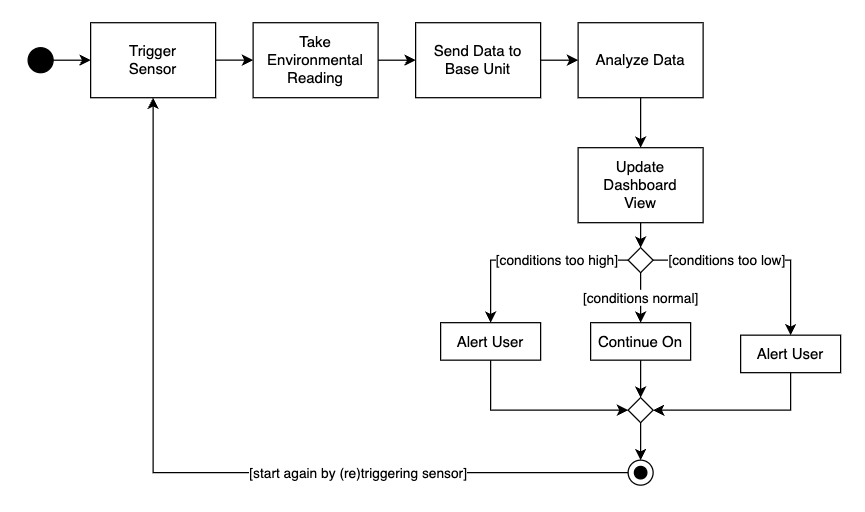
\includegraphics[scale=.35]{images/AD.png}
    \end{center}
  \end{frame}

  \begin{frame}{\sectitle}{Requirements -- Abbreviated}
    Sensor:
    \begin{itemize}\scriptsize
      \item Sensor(s) shall be capable of taking and recording temperature and humidity readings.
      \item Sensor(s) shall transmit readings back to the base unit in a usable data form.
    \end{itemize}
    \vspace*{.5em}
    Base Unit:
    \begin{itemize}\scriptsize
      \item The base unit shall host the server for the web interface.
      \item The base unit shall posess data analysis capabilities.
    \end{itemize}
    \vspace*{.5em}
    Web Interface:
    \begin{itemize}\scriptsize
      \item Users shall be able to set upper and lower bounds for acceptable temperatures and humidity ranges.
      \item The web interface shall send a notification if either temperature or humidity drift out of the established acceptable range.
    \end{itemize}
  \end{frame}


  \renewcommand{\sectitle}{Mockups}
  \section{\sectitle}
  \begin{frame}{Roadmap}
    \tableofcontents[currentsection]
  \end{frame}

  \begin{frame}{\sectitle}{Sensor Overview Page}
    \begin{center}
      \frame{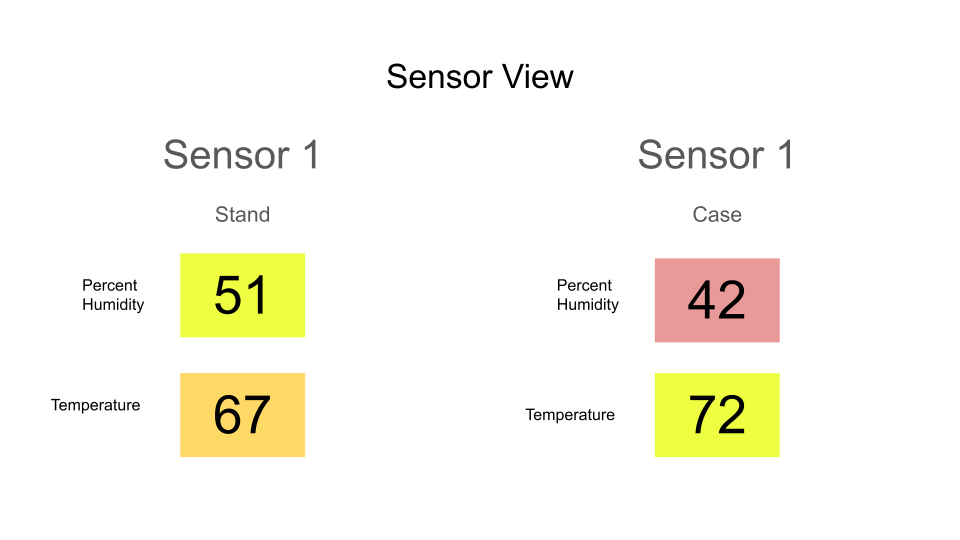
\includegraphics[scale=.3]{images/sensor-overview.png}}
    \end{center}
  \end{frame}

  \begin{frame}{\sectitle}{Sensor Detail Page}
    \begin{center}
      \frame{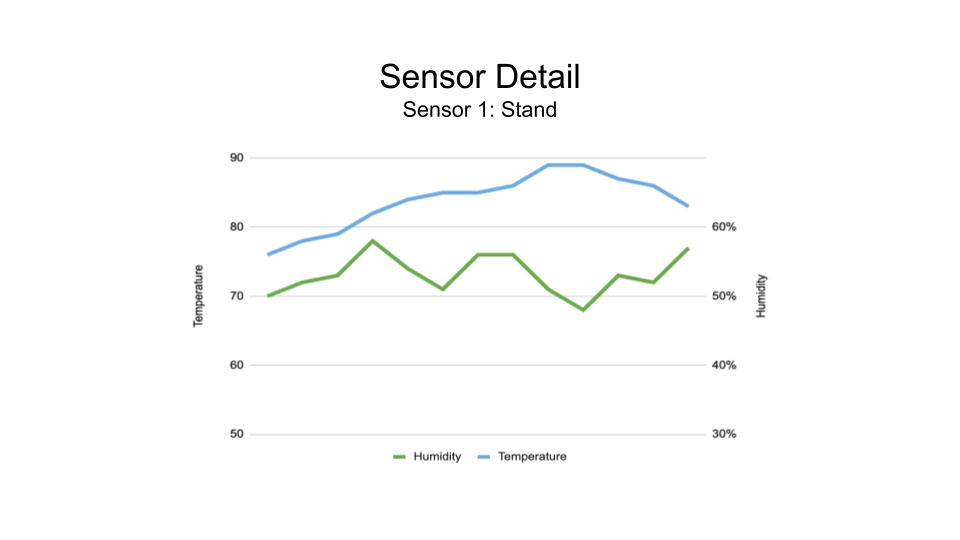
\includegraphics[scale=.3]{images/sensor-detail.png}}
    \end{center}
  \end{frame}

  \begin{frame}{\sectitle}{Sensor Management Page}
    \begin{center}
      \frame{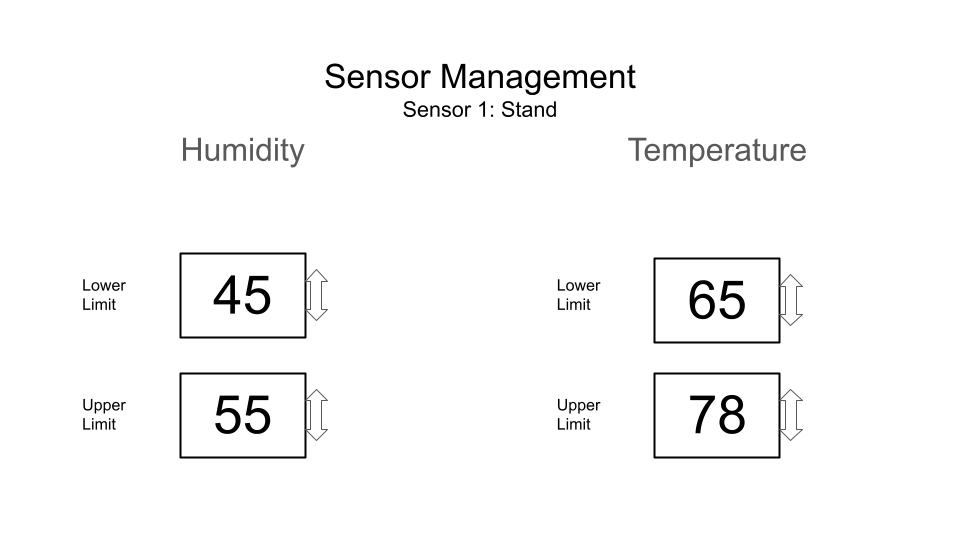
\includegraphics[scale=.3]{images/sensor-management.png}}
    \end{center}
  \end{frame}


\end{document}